\documentclass{beamer}

%%% SOLARIZED THEME %%%
\usecolortheme[light, accent=orange]{solarized}

%%% PACKAGES %%%
\usepackage{graphics}
\usepackage{booktabs}
\usepackage{standalone}
\usepackage{tikz}
\usetikzlibrary{positioning, arrows}

%%% TITLE %%%
\title{\textsc{A cool presentation}}
\author{Nikoleta E. Glynatsi}
\date{}

\begin{document}
    \maketitle

    \begin{frame}
        \centering
        \Huge HUGE
    \end{frame}

    \begin{frame}
        \centering
        \Huge \textcolor{solarizedRed}{HUGE}
    \end{frame}

    \begin{frame}
        \centering
        \Huge \textbf{HUGE}
    \end{frame}

    \begin{frame}
        \centering
        \begin{itemize}
            \item Awesome result one
            \item Awesome result two
            \item Awesome result three
        \end{itemize}
    \end{frame}

    \begin{frame}
        \centering
        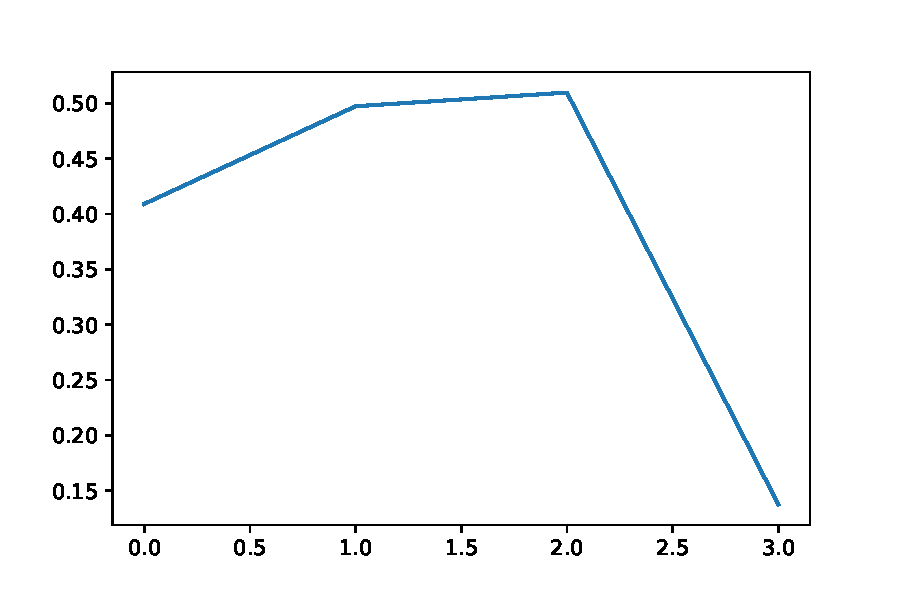
\includegraphics[width=.7\textwidth]{lineplot.pdf}
    \end{frame}

    \begin{frame}
        \centering
        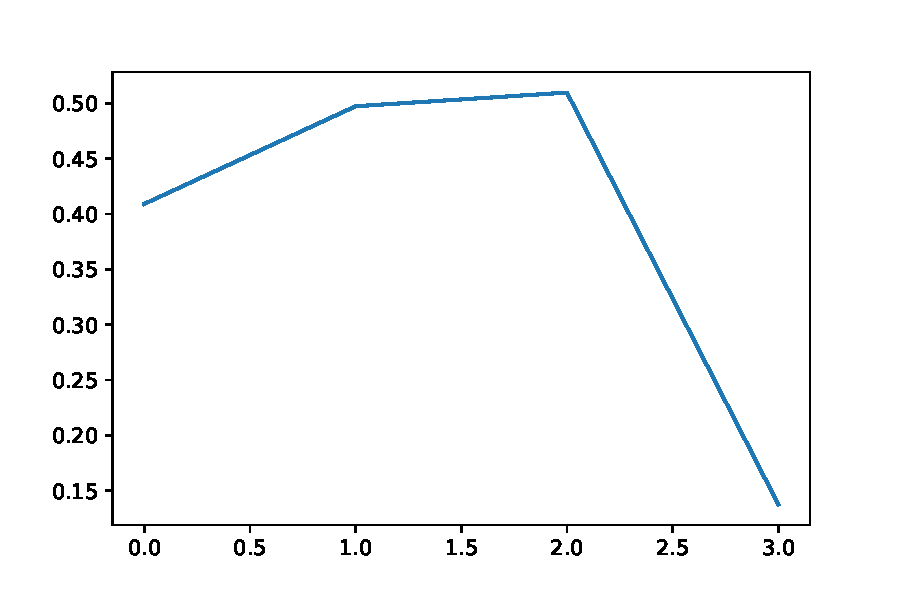
\includegraphics[width=.45\textwidth]{lineplot.pdf} 
        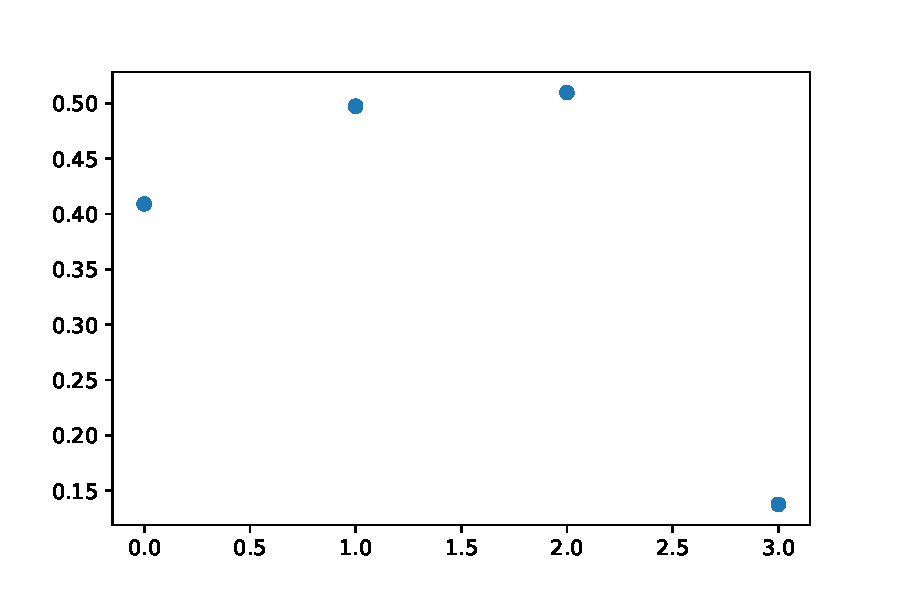
\includegraphics[width=.45\textwidth]{scatter.pdf}
    \end{frame}

    \begin{frame}
        \begin{minipage}{0.49\textwidth}
            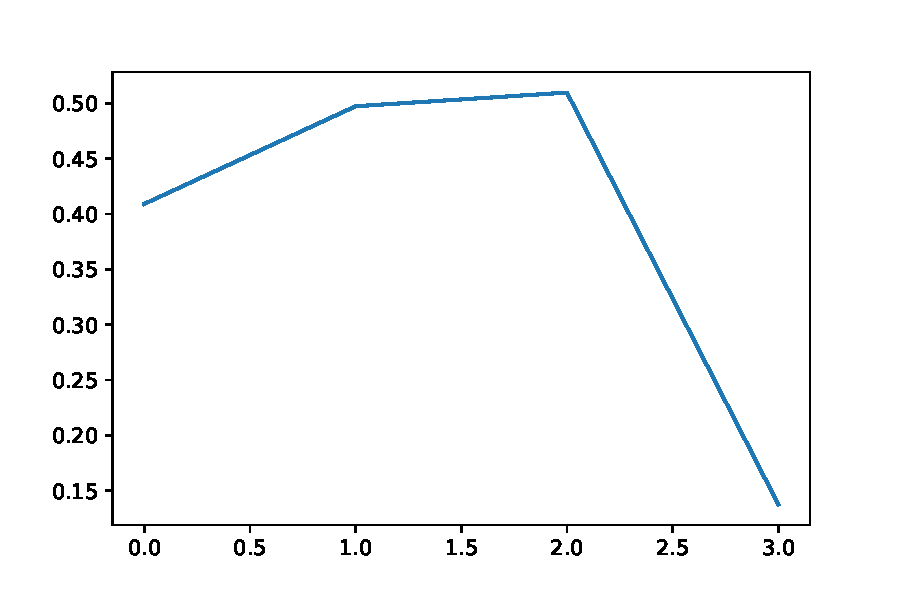
\includegraphics[width=\textwidth]{lineplot.pdf} 
        \end{minipage}
        \begin{minipage}{0.49\textwidth}
            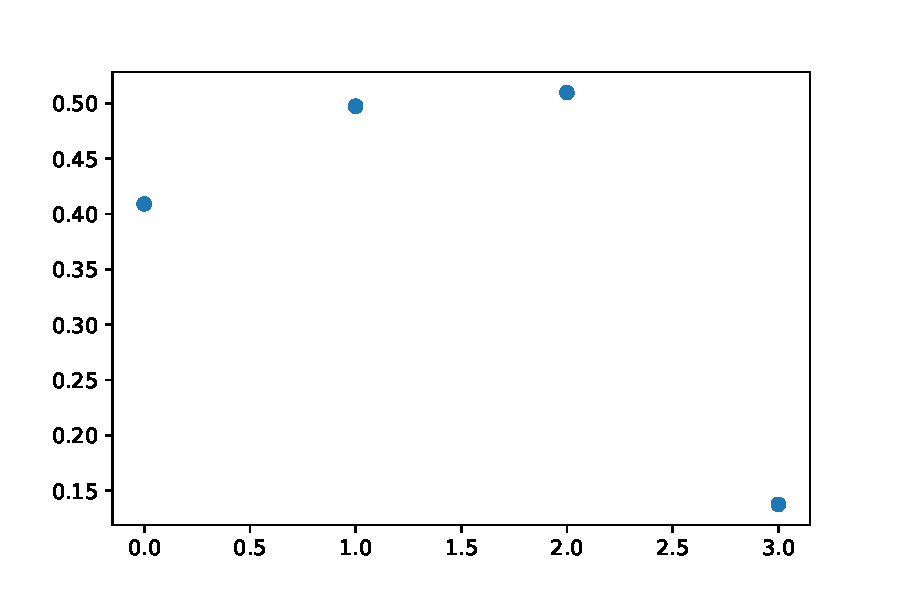
\includegraphics[width=\textwidth]{scatter.pdf}
        \end{minipage}
    \end{frame}

    \begin{frame}
        \begin{minipage}{0.49\textwidth}
            \centering
            \Huge HUGE
        \end{minipage}
        \pause
        \vspace{1cm}
        \begin{minipage}{0.49\textwidth}
            \centering
            \small SMALL
        \end{minipage}
    \end{frame}

    \begin{frame}
        \centering
        \documentclass{standalone}
    \usepackage{tikz}
    \usepackage{xcolor}
    \definecolor{plain}{rgb}{93,93,93}
    \usetikzlibrary{positioning,arrows, calc, arrows.meta}
    
    \definecolor{applegreen}{rgb}{0.55, 0.71, 0.0}
    \begin{document}
    \tikzset{man/.pic={
        \node[circle,fill,minimum size=5mm] (head) {};
        \node[rounded corners=2pt,minimum height=.8cm,minimum width=0.4cm,fill,below = 1pt of head] (body) {};
        \draw[line width=1mm,round cap-round cap] ([shift={(2pt,-1pt)}]body.north east) --++(-90:6mm);
        \draw[line width=1mm,round cap-round cap] ([shift={(-2pt,-1pt)}]body.north west)--++(-90:6mm);
        }}
    \tikzset{big_man/.pic={
        \node[circle,fill,minimum size=3mm] (head) {};
        \node[circle,left = -15pt of head, fill,minimum size=5mm] (head_2) {};
        \node[circle,right = -15pt of head, fill,minimum size=5mm] (head_3) {};
        \node[draw=solarizedBase03, circle,fill,minimum size=5mm] (head) {};
         \node[rounded corners=2pt,minimum height=.8cm,minimum width=0.4cm,fill,below = 1pt of head] (body) {};
        \draw[line width=1mm,round cap-round cap] ([shift={(2pt,-1pt)}]body.north east) --++(-90:6mm);
        \draw[line width=1mm,round cap-round cap] ([shift={(-2pt,-1pt)}]body.north west)--++(-90:6mm);
        }}
    \tikzset{small_man/.pic={
            \node[circle,fill,minimum size=2.5mm] (head) {};
            \node[rounded corners=2pt,minimum height=.4cm,minimum width=0.2cm,fill,below = .5pt of head] (body) {};
            \draw[line width=.5mm,round cap-round cap] ([shift={(1pt,-.5pt)}]body.north east) --++(-90:3mm);
            \draw[line width=.5mm,round cap-round cap] ([shift={(-1pt,-.5pt)}]body.north west)--++(-90:3mm);
            }}
    \tikzset{cloud/.pic={
                \node[cloud, cloud puffs=10.8,minimum width=1cm, minimum height=1.1cm, draw] () at (0,0) {\tikzpictext};
                }}
    \begin{tikzpicture}
        \pic[solarizedRed] at (0, .5) (myman) {man};
        \pic[solarizedBlue] at (0, -2) (myman) {man};
        \pic at (-.8, -1) (myman) {small_man};
        \pic at (-.8, -1.2) (cloud) {cloud};
        \node at (-.25, -1.75) [circle,fill,inner sep=1pt] {};
        \node at (-.35, -1.65) [circle,fill,inner sep=1pt] {};


        \pic[solarizedGreen] at (0, -4.5) (myman) {big_man};
        \pic at (-.8, -3.4) (myman) {small_man};
        \pic at (-.8, -3.6) (cloud) {cloud};
        \node at (-.25, -4.15) [circle,fill,inner sep=1pt] {};
        \node at (-.35, -4.05) [circle,fill,inner sep=1pt] {};


        \node (0) at (4, 0) {$\bullet$ ZD strategies are not adaptable.};
        \node (1) at (3.4, -2.5) {$\bullet$ Extortion is not optimal.};
        \node (2) at (3.7, -5) {$\bullet$ Longer memory is beneficial.};

    \end{tikzpicture}
    \end{document}
    \end{frame}

    \begin{frame}
        \centering
        \includestandalone[width=.7\textwidth]{game}
    \end{frame}

    \begin{frame}
    \centering

    Nikoleta \\ glynatsi@evolbio.mpg.de \\

    \vspace{1cm}
    \small{http://web.evolbio.mpg.de/social-behaviour/}
    
    \end{frame}

\end{document}